\documentclass[a4paper,10pt]{article}

%%%%%%%%%%%% PREÁMBULO %%%%%%%%%%%%%%%%%%%%%

% Paquetes

\usepackage[utf8]{inputenc}
\usepackage[spanish,es-tabla]{babel}
\usepackage[T1]{fontenc}
\usepackage{graphicx}

\usepackage{listings}

% Comandos

\renewcommand{\lstlistingname}{Código}
\renewcommand{\lstlistlistingname}{Índice de fragmentos de código fuente}

% Opciones

\title{Empresas para MongoFallero}
\author{Angel Berlanas Vicente}

%%%%%%%%%%%%%%%%%%%%%%%%%%%%%%%%%%%%%%%%%%%%%%

\begin{document}
\maketitle

\begin{abstract}
Resumen de las diferentes característica y requisitos de las tres empresas que participan en el contrato de MongoFallero. 
\end{abstract}

\tableofcontents

\section{Requisitos Generales}

\begin{itemize}
    \item Lenguajes
    \item Herramientas
    \item Mobile First
    \item Comentarios
\end{itemize}

\subsection{Lenguajes}

Para la realización de las hojas de estilo que aplicarán a nuestra aplicación de MongoFallero debemos contar con el uso de \textit{SaSS} que nos permitirá realizar las hojas de estilo necesarias para adecuarnos a las tres empresas ganadoras y aplicar tan solo aquella que se desee en el momento del exámen (quería decir \textit{venta del producto}). De tal manera que tendremos que tener preparados los estilos haciendo uso de las posibilidades que nos da \textit{SaSS} para poder obtener esta flexibilidad.

A continuación se detallan los requisitos de diseño de cada una de las tres empresas que pugnan por la aplicación, debemos de ser capaces de modificando \textit{una sola variable} en el \texttt{.scss}.

Durante la evaluación del ejercicio se pedirá que se modifique esa \texttt{variable} y que se recompilen los ficheros \texttt{css} con ayuda de \textit{SaSS}, o cualquier variación de esto:

\begin{itemize}
\item Ejecución de \texttt{ruby-sass} manualmente.
\item El uso sass con la opción de \textit{vigilancia} para estar pendiente de los cambios.
\item Configuración del módulo de \textit{nodejs} de \texttt{node-sass}.
\item Otras propuestas por el alumnado.
\end{itemize}

Una vez compilado de forma ágil y \textit{sin errores} el profesor pasará a comprobar que todos los requisitos definidos en este documento han sido cubierto para todas las empresas. Esto no significa que revise \textbf{todas}, pero si que \textit{puede hacerlo}.

Recordad que el objetivo de esta actividad es demostrar que \textit{habéis aprendido} y que tenéis las destrezas necesarias.

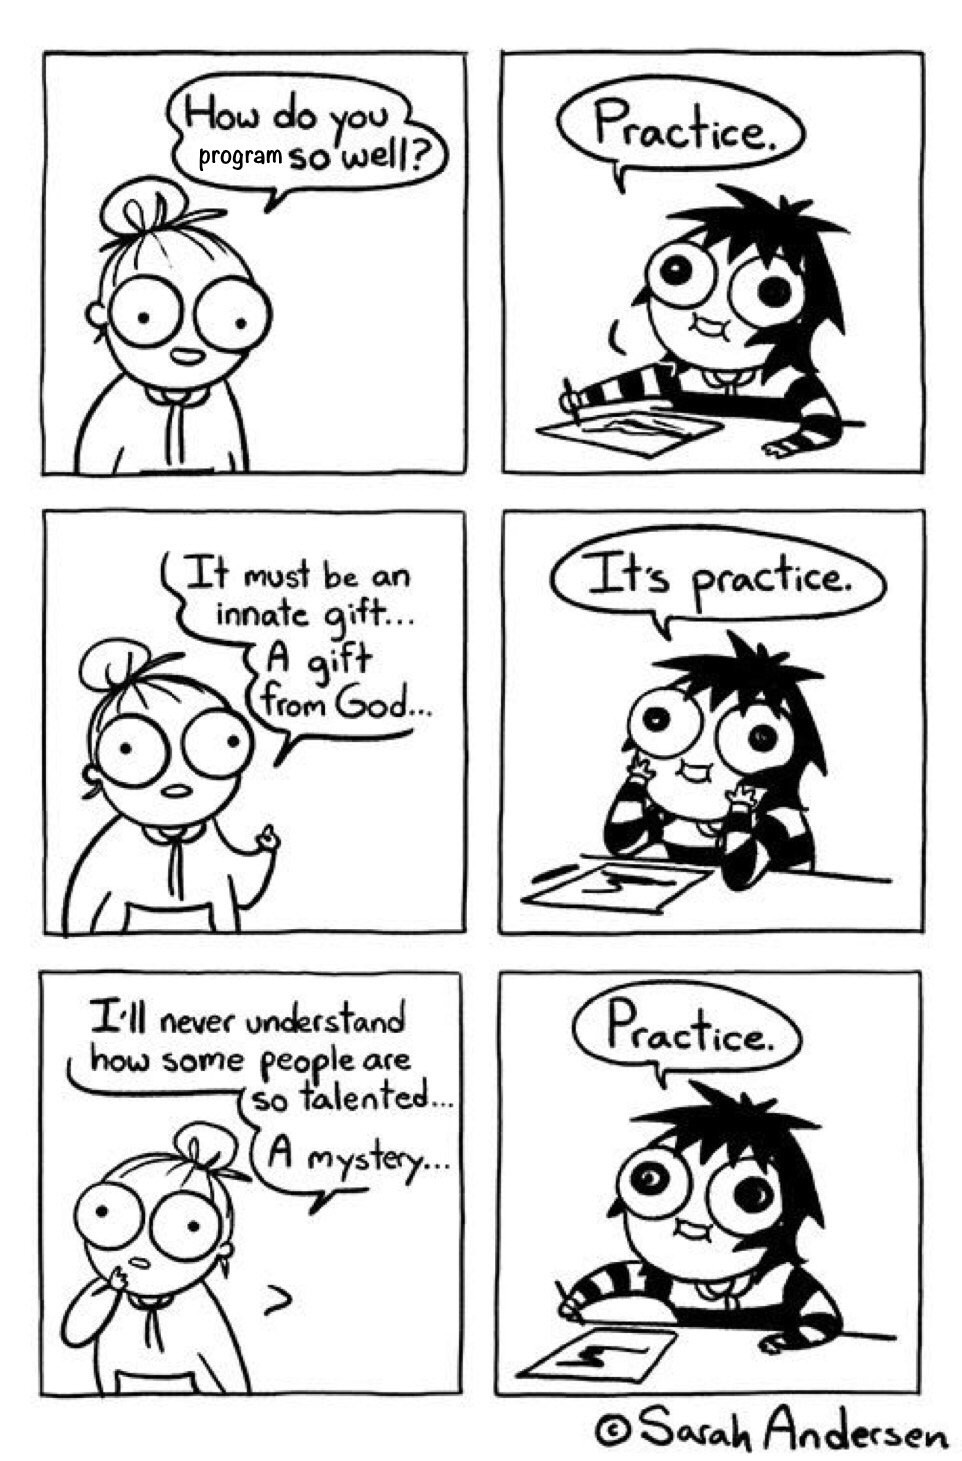
\includegraphics{imgs/practice}

\end{document}
